\section{iQAQE Schemes and Results}
\label{sec:concl}

% Maybe re-read what I have until here, before resuming writing.

Now, we present the various iQAQE schemes we have developed and the results of their numerical simulations. For a more detailed discussion, please refer to the full thesis (Chapter 5). Keep in mind that all numerical results refer to the same $8$-node graph: \texttt{\myurl{E = [(0, 1), (0, 2), (0, 6), (1, 2), (1, 6), (3, 2), (3, 4), (3, 5), (4, 5), (4, 7), (5, 7), (6, 7)]}}.


% \begin{figure}[t]
%     \centering
%     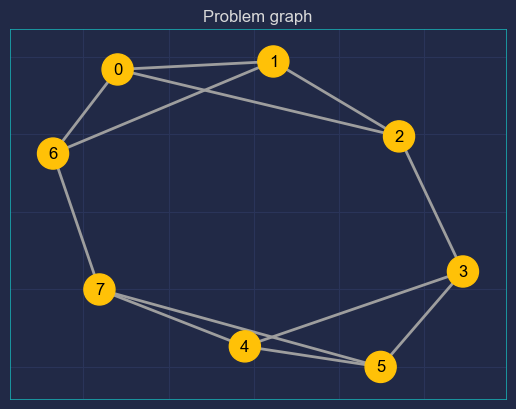
\includegraphics[width=0.95\columnwidth]{Figures/problem_graph.png}
%     \caption{Considered $8$-node graph instance. The optimal cut ($10$) was found through
%     brute-force (exhaustive search).}
%     \label{fig:8_node_graph}
% \end{figure}

\subsection{Random iQAQE}
\label{subsec:Random_iQAQE}

First and foremost, we aim to understand how iQAQE compares with both QAOA and QEMC. For this comparison, $n$ and $c$ were randomly chosen ($n = c = 4$). Currently, the allocation of basis states to lists is also done randomly. The goal of this initial simulation is to take a preliminary look at iQAQE's performance and understand how much the results vary between finite shot number simulations and analytical ones (Figure \ref{fig:3_Comparison_shots}). These plots generally align with our theoretical expectations. As QEMC relies heavily on a large number of shots, transitioning to a finite shot number naturally impacts the results. Surprisingly, however, iQAQE seems to exhibit slightly greater resilience to this effect, despite sharing QEMC's cost function and ansatz. This resilience might be attributed to the presence of multiple basis states associated with each graph node, potentially reducing the need for exhaustive sampling.

% Chapter 5's figure. Positioning!
\begin{figure*}[t]
    \centering
    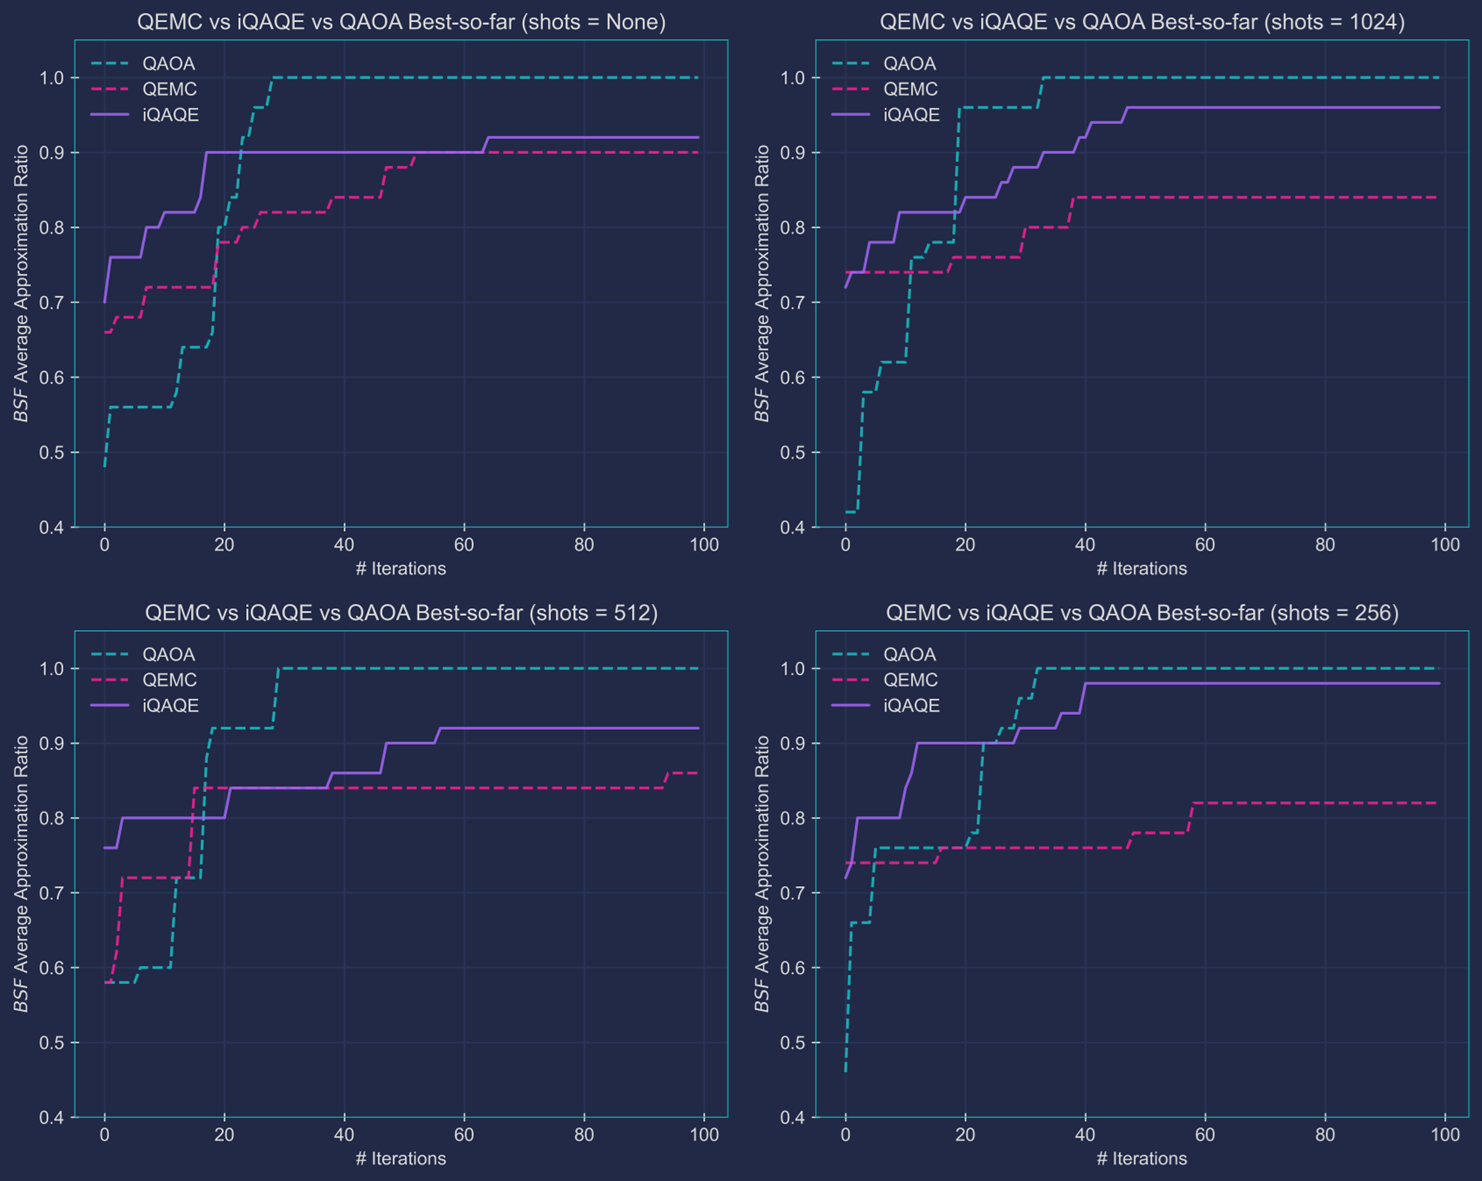
\includegraphics[width=0.90\textwidth]{Figures/Random_iQAQE_Updated.png}
    \caption{Comparison between the $3$ VQAs' performances (QAOA, QEMC and iQAQE), using an infinite and finite number of shots. The best-so-far average is plotted ($8$-node graph).}
    \label{fig:3_Comparison_shots}
\end{figure*}

\subsection{Polynomial Compression-type Encodings}
\label{subsection:Polynomial_Encodings}
These schemes fix one or more qubits to $1$ (or $0$) while letting the others vary\footnote{Fixing qubits means we only permit basis states where certain qubits are set to either $0$ or $1$. Each node has specific qubits fixed, and these fixed qubits differ between nodes, forming the basis for our mappings.}. Fixing $k$ qubits achieves polynomial compression of order $k$. The total number of nodes encoded is $\binom{n}{k}$, the number of ways to select $k$ qubits from $n$. We select the smallest $n$ such that $\binom{n}{k} \geq N$, resulting in $N = \mathcal{O}(n^k)$. We then decide how many basis states to use for each node, chosen from $2^{n-k}$. We may use all $2^{n-k}$ states or choose a subset $c \leq 2^{n-k}$. Upon selecting the mapping, the algorithm uses QEMC's cost function and ansatz. Polynomial compression ensures $n < N$ unless $k = 1$.

\subsubsection{Basic Polynomial Compression-type iQAQE}
\label{subsubsection:Basic_Polynomial_iQAQE}
\vspace{-2.5mm}
\begin{figure}[H]
    \centering
    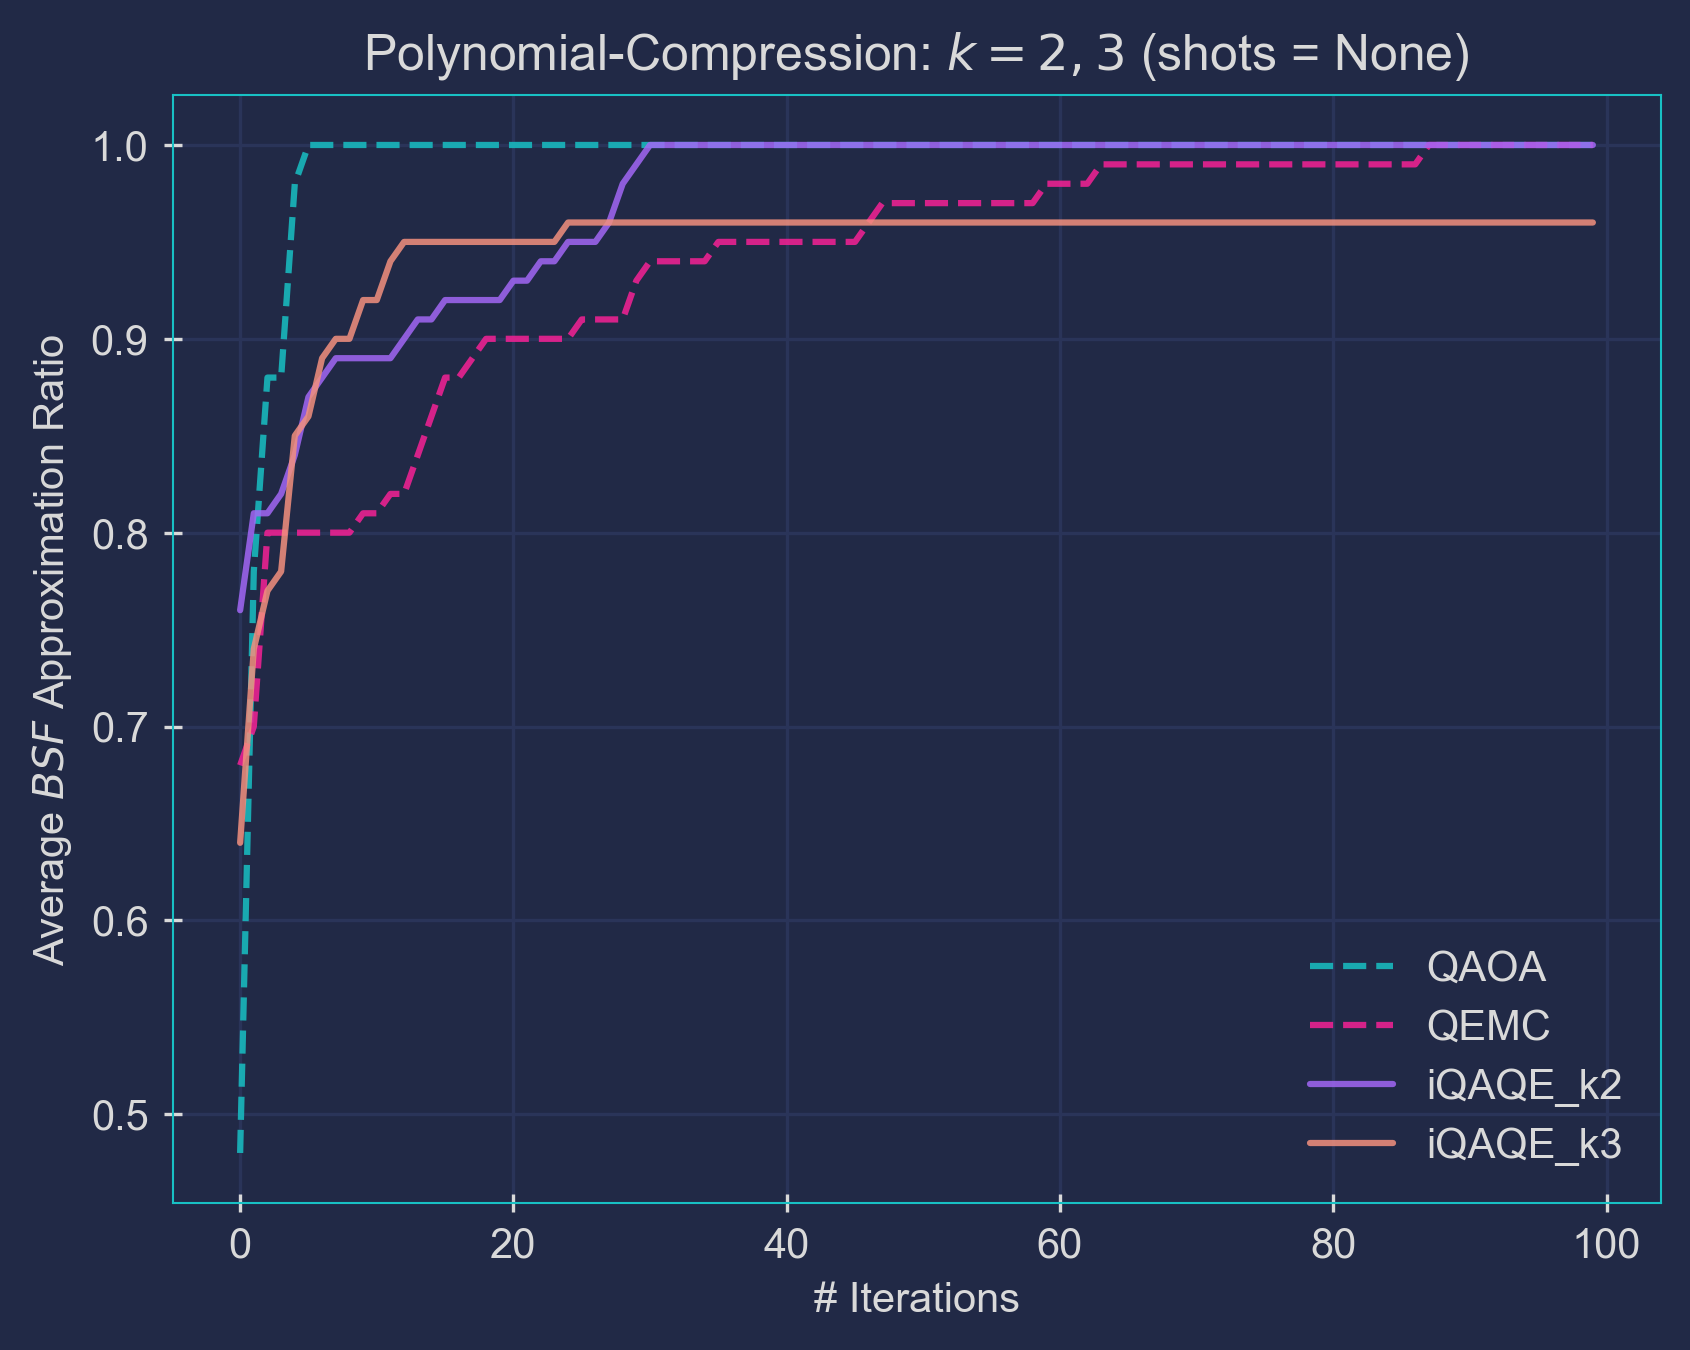
\includegraphics[width=0.95\columnwidth]{Figures/Polynomial_Compression_Base_k2_k3_1.png}
    \caption{Average BSF Approximation Ratio \textit{vs.} iteration number for the tested VQAs. The number of layers considered were $4$ for $k = 2$ and $5$ for $k = 3$ ($8$-node graph).}
    \label{fig:Comparison_k2+k3_2}
\end{figure}
\vspace{-3.5mm}
This is the simplest type of polynomial compression-based iQAQE scheme. It involves fixing $k$ qubits to $1$ instead of $0$ (e.g., $\{\ket{11\text{xxx}}\}$, for $k = 2$). The number of fixed qubits ($k$) is determined by the desired order of compression, as previously described. The results for $k = 2$ and $k = 3$ are shown in Figure \ref{fig:Comparison_k2+k3_2}. Results-wise, \texttt{iQAQE\_k2} achieves a perfect average BSF approximation ratio, although it requires more iterations than QAOA. Our method outperforms QEMC for $k = 2$, but yields less promising results for $k = 3$. Nevertheless, both mappings use fewer qubits ($n = 5$) compared to QAOA ($n = 8$), which is advantageous for implementation on practical (NISQ) quantum computers.

\subsubsection{Correlation-based iQAQE}
\label{subsubsection:Correlation_iQAQE}

This scheme closely resembles what was previously discussed in subsection \ref{subsubsection:Basic_Polynomial_iQAQE}. The key distinction lies in the inclusion of the possibility for both $0$'s and $1$'s to be fixed (e.g., $\{\ket{11\text{xxx}}, \ket{00\text{xxx}}\}$, for $k = 2$; recall, this encodes a single node). Consequently, the scheme aims to identify correlations among the different qubits, wherein "correlations" denote identical colors. This approach was inspired by the notion that by identifying correlations between nodes, it becomes feasible to color the entire graph as long as one node is initially colored. We present the results of numerical simulations applied to the standard $8$-node graph using this correlation-based iQAQE approach (Figure \ref{fig:Correlation/k=2,3,4}).

% Removed!
% In other words, the constructed lists regard the $k$ fixed qubits as positively correlated, meaning they are either all set to $1$ or all set to $0$.

% Also removed!
% Although seeking correlations between qubits, as done here, differs from seeking correlations between nodes, we anticipated that it might yield promising results to some extent. In this scenario, the color of each node is determined by the probability that its $k$ associated qubits are all positively correlated.

\begin{figure}[H]
    \centering
    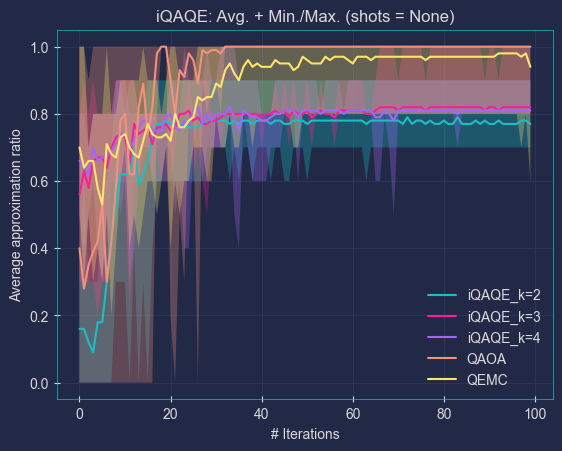
\includegraphics[width=0.95\columnwidth]{Figures/Correlation-based/k=2_3_4.png}
    \caption{Comparison of correlation-based iQAQE results for $k=2, 3$, and $4$ with outcomes from QAOA and QEMC ($8$-node graph).}
    \label{fig:Correlation/k=2,3,4}
\end{figure}

The underperformance may stem from doubling the number of basis states in each sub-list, resulting in a $50\%$ overlap between pairs of sub-lists, akin to Basic Polynomial Compression-type iQAQE. However, this time, with twice the basis states, the (absolute) overlap is significantly higher, leading to more shared states among nodes. When overlap is excessive, adjusting one node's color without affecting others becomes more challenging, likely causing the underperformance.

\subsubsection{Fixed-Parity iQAQE}
\label{subsubsection:Fixed-Parity_iQAQE}

Now, we present another heuristic method for mapping the basis states to the nodes. Although it is similar to the previous one, this time we fixed the parity of the selected $k$ qubits to be even. Parity is determined by the number of $1$'s: if the count is even, the parity is even; otherwise, it is odd. For instance, for $k=3$ (with \texttt{n\_qubits = 5}), the lists would take the form: (Keep in mind that we are using an $8$-node graph.)
% \vspace{-10mm}
% Remeber that 'k=2' is the same as the previous correlation-based! Mention this in the text!
{\normalsize\begin{enumerate}[itemsep=0mm]
    \item $\left\{\ket{000\text{xx}}, \ket{011\text{xx}}, \ket{101\text{xx}}, \ket{110\text{xx}}\right\}$;
    \item $\left\{\ket{00\text{xx}0}, \ket{01\text{xx}1}, \ket{10\text{xx}1}, \ket{11\text{xx}0}\right\}$;
    \item $\left\{\ket{0\text{xx}00}, \ket{0\text{xx}11}, \ket{1\text{xx}01}, \ket{1\text{xx}10}\right\}$;
    \item $\left\{\ket{\text{xx}000}, \ket{\text{xx}011}, \ket{\text{xx}101}, \ket{\text{xx}110}\right\}$, etc.
\end{enumerate}} % \vspace{-10mm}
\noindent We have presented only the first four nodes. Numerical simulations were performed, and the obtained results are presented in Figure \ref{fig:Fixed-parity/k=2,3,4}. While performance still lags behind QAOA, it is notably better than the previous scenario. For $k=2$, the results match the previous correlation-based scheme, as requiring pairs to be even is equivalent to requiring them to be the same.
% \vspace{-10mm}
\begin{figure}[H]
    \centering
    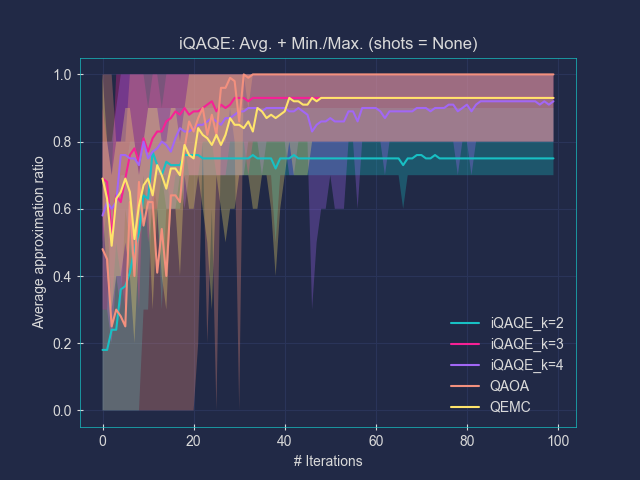
\includegraphics[width=0.95\columnwidth]{Figures/Fixed-parity/k=2_3_4(8-node).png}
    \caption{Fixed-parity iQAQE for $k=2, 3$, and $4$ compared with the results from QAOA and QEMC ($8$-node graph).}
    \label{fig:Fixed-parity/k=2,3,4}
\end{figure}
% \vspace{-10mm}

\subsection{Unmodified Extended-QEMC}
\label{subsection:Vanilla_Extended_QEMC}

\begin{figure}[H]
    \centering
    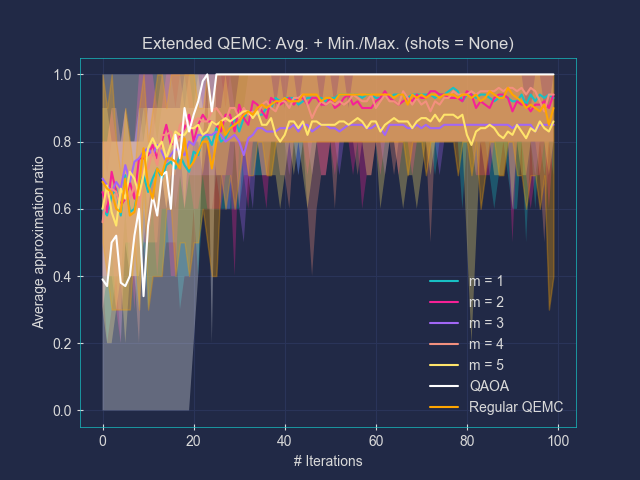
\includegraphics[width=0.95\columnwidth]{Figures/Extended-QEMC/8-node(n_layers=3, step_size=0.95, m=All).png}
    \caption{Implementation of the Unmodified Extended-QEMC scheme for the usual $8$-node graph: comparison with QAOA and regular QEMC for various values of $m$. Note that $m$ is not extended beyond $5$, as this would exceed the number of qubits used in QAOA. Additionally, we utilize \texttt{n\_layers = 3}, \texttt{step\_size = 0.95} and \texttt{B = 4}.}
    \label{fig:Vanilla_Extended-QEMC}
\end{figure}

Amid the various schemes we've attempted, I've devised an extension to the standard QEMC scheme. This new approach enhances QEMC by incorporating $m$ additional qubits beyond the usual $\lceil\log_2(n)\rceil$ qubits required for $n$ graph nodes. This increase in qubits prevents the scheme from being easily classically simulable and allows for more basis states to be associated with each graph node. This scheme assigns $2^m$ basis states per node. Importantly, similar to QEMC, the sets of basis states associated with different nodes do not overlap. The assignment of states to each list is currently arbitrary. For simplicity, we use a straightforward partition: the first $2^m$ basis states go to the first list, the next $2^m$ to the second list, and so on. Now, I present the results of applying this scheme to the usual $8$-node graph (Figure \ref{fig:Vanilla_Extended-QEMC}).

\subsection{Alternative ansätze}
\label{subsection:Alternative_Ansätze}
After considering whether QEMC and iQAQE could be affected by a generic ansatz, I pondered if tailored ansätze and excess entanglement might impact performance. To address this, I proposed implementing non-deterministic CNOT gates (ND-CNOTs\footnote{We recognize that the term "non-deterministic CNOT gates" is employed in linear optical quantum computing (KLM protocol), yet we use it differently in this context.}), adjusting entanglement dynamically. We achieved this by adding parameterized $R_x$ gates before each CNOT's control qubit. Following numerical testing, we discovered that despite increasing complexity in the optimization landscape, this seems to substantially improve performance, especially when coupled to QEMC.

\subsection{Goemans-Williamson and Bigger Graphs}
\label{subsection:GW_Bigger_Graphs}

\begin{figure}[H]
    \centering
    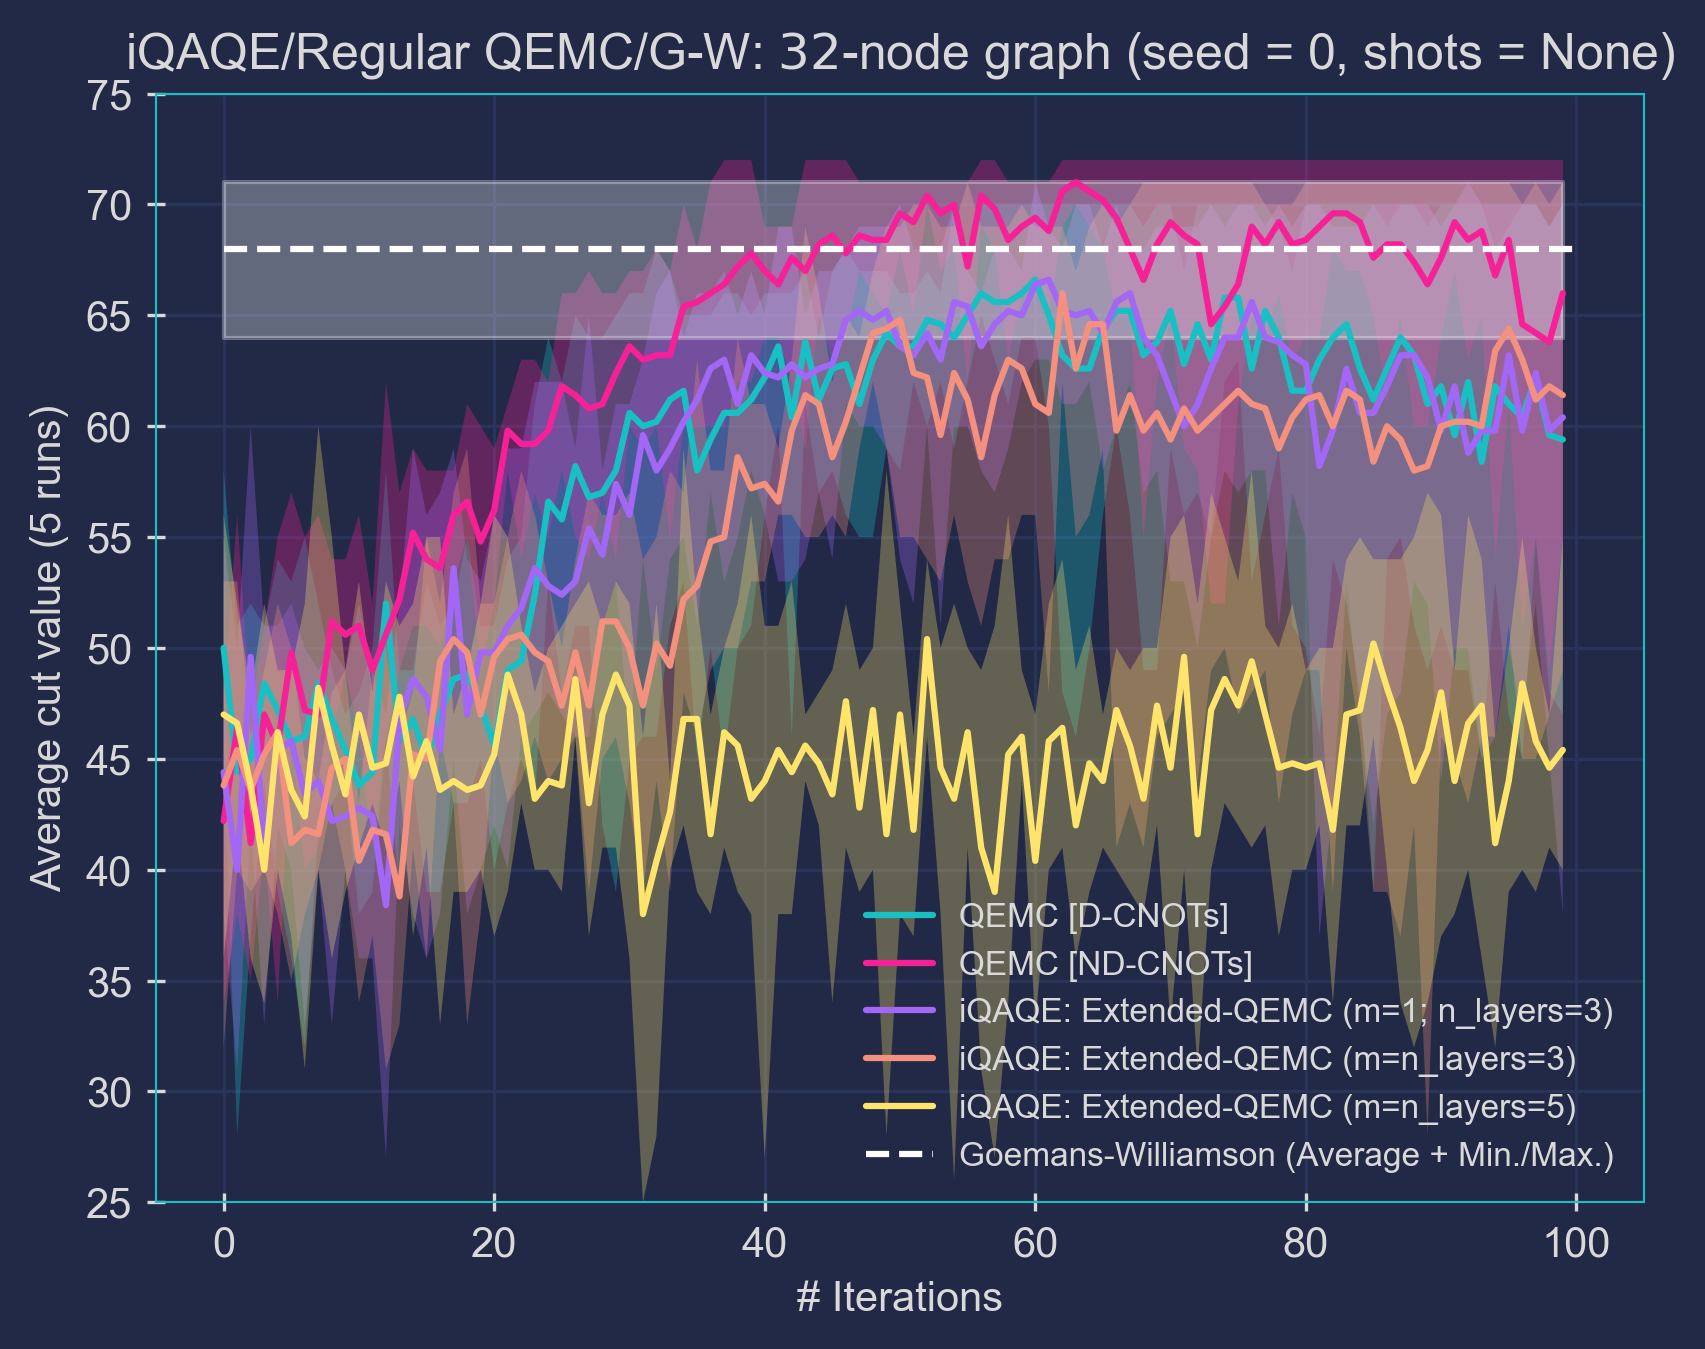
\includegraphics[width=0.95\columnwidth]{Figures/Large graphs/32-node_Graph_seed=0.png}
    \caption{Comparison of performance (average cut values) among various VQAs for a $32$-node graph.}
    \label{fig:32-node_Graph}
\end{figure}

To assess the scalability of these algorithms, we conducted tests on larger graphs, facilitating more accurate comparisons with classical state-of-the-art methods (GW). The results ($32$-node graph) for the most promising algorithms are depicted in Figure \ref{fig:32-node_Graph}. Remarkably, the average performance of ND-CNOT-based QEMC competes closely with GW, occasionally surpassing it. Moreover, the maximum performance of the same ND-CNOT QEMC exceeds that of GW, as seen in Figure \ref{fig:32-node_Graph} (shaded regions). This marks the first instance in our study where one of our heuristics outperforms classical state-of-the-art algorithms, highlighting significant progress and indicating the potential for further exploration within the proposed iQAQE Framework. Other heuristics were explored in this project but are not included here due to space limitations. We have presented the most significant results, though all findings are important and should not be overlooked. For a thorough discussion, please consult the full thesis (Chapter 5).

\subsection{Randomized iQAQE benchmarking -- Machine learning-based approach}
\label{subsection:Randomized_iQAQE_ML}
We also proposed a scheme for determining the optimal mapping for a specific graph based on statistical properties of the mappings themselves, using a small machine learning model. Such a model necessitates defining input (independent variables - IVs) and output (dependent variable - DV). Our IVs will encompass statistically significant properties\footnote{Examples: number of basis states, average Hamming weight, average pair-wise Hamming distance, etc.} extracted from each node's specific sub-list. Alternatively, including the basis states' mapping directly as the model's input presents challenges concerning memory-efficient encoding. Traditional one-hot encoding methods are inadequate due to the vast number of potential basis states available (which scales exponentially with the number of qubits). Additionally, the median BSF cut value after training was selected as the DV. Initially, we utilized a multiple linear regression model. Upon observing significant multicollinearity among some IVs, we transitioned to principal component analysis (PCA), followed by regression (PCR). Although the results were not entirely satisfactory, we believe this approach can inspire future research, building on this idea and our initial work. For a more detailed discussion, please refer to the full thesis (Chapter 5).